% preview.tex — Stand-alone preview version (no IEEEtran required)
% Use this if pdflatex is available locally but IEEEtran.cls is not installed.
% For the final submission-quality PDF, compile main.tex in Overleaf.
%
% Compile: pdflatex preview.tex && bibtex preview && pdflatex preview.tex && pdflatex preview.tex

\documentclass[twocolumn,10pt]{article}

\usepackage[letterpaper,
            top=1in, bottom=1in,
            left=0.75in, right=0.75in,
            columnsep=0.5in]{geometry}

\usepackage{times}           % Times New Roman equivalent
\usepackage{cite}
\usepackage{amsmath}
\usepackage{amssymb}
\usepackage{graphicx}
\usepackage{booktabs}
\usepackage{multirow}
\usepackage{url}
\usepackage{hyperref}
\usepackage{microtype}
\usepackage{titlesec}
\usepackage{abstract}

%% ---- Mimic IEEE section style --------------------------------
\titleformat{\section}{\normalfont\bfseries\scshape\centering}{}{0em}{}
\titlespacing{\section}{0pt}{6pt}{3pt}
\titleformat{\subsection}{\normalfont\itshape}{}{0em}{}
\titlespacing{\subsection}{0pt}{4pt}{2pt}

%% ---- Figure path ---------------------------------------------
\graphicspath{{figures/}}

%% ---- Numerical macros ----------------------------------------
% AUTO-GENERATED by scripts/make_paper_numbers.py — do not edit by hand
% Usage in LaTeX: \N{QualC} expands to 3.47

\newcommand{\N{NpromptTotal}}{50}
\newcommand{\N{NpromptCS}}{25}
\newcommand{\N{NpromptBio}}{25}
\newcommand{\N{NseedsReported}}{5}
\newcommand{\N{QualA}}{3.08}
\newcommand{\N{QualAlo}}{2.91}
\newcommand{\N{QualAhi}}{3.26}
\newcommand{\N{NovA}}{0.41}
\newcommand{\N{DivA}}{0.38}
\newcommand{\N{GroundA}}{71.4\%}
\newcommand{\N{TokensA}}{487}
\newcommand{\N{QualB}}{3.31}
\newcommand{\N{QualBlo}}{3.14}
\newcommand{\N{QualBhi}}{3.48}
\newcommand{\N{NovB}}{0.43}
\newcommand{\N{DivB}}{0.41}
\newcommand{\N{GroundB}}{73.6\%}
\newcommand{\N{TokensB}}{2{,}435}
\newcommand{\N{QualC}}{3.47}
\newcommand{\N{QualClo}}{3.29}
\newcommand{\N{QualChi}}{3.64}
\newcommand{\N{NovC}}{0.46}
\newcommand{\N{DivC}}{0.52}
\newcommand{\N{GroundC}}{76.8\%}
\newcommand{\N{TokensC}}{4{,}122}
\newcommand{\N{DeltaQ}}{0.39}
\newcommand{\N{DeltaDiv}}{0.14}
\newcommand{\N{DeltaNov}}{0.05}
\newcommand{\N{TokenRatio}}{3.4\times}
\newcommand{\N{SCGapClose}}{59\%}
\newcommand{\N{MADSuccess}}{80\%}
\newcommand{\N{MADHalluc}}{12\%}
\newcommand{\N{MADFalse}}{8\%}
\newcommand{\N{QualACS}}{3.11}
\newcommand{\N{QualCCS}}{3.52}
\newcommand{\N{QualABio}}{3.05}
\newcommand{\N{QualCBio}}{3.42}
\newcommand{\N{QualRound1}}{3.38}
\newcommand{\N{TokensRound1}}{2{,}890}
\newcommand{\N{QualRound2}}{3.47}
\newcommand{\N{TokensRound2}}{4{,}122}
\newcommand{\N{QualRound3}}{3.44}
\newcommand{\N{TokensRound3}}{5{,}980}


%% ==============================================================
\begin{document}

\twocolumn[{%
  \centering
  {\Large\bfseries Does Debate Improve Scientific Hypothesis Quality?\\[4pt]
    A Comparative Study of Single-LLM, Self-Consistency,\\
    and Multi-Agent Debate on HypoBench}\\[8pt]
  {\normalsize Subhadip Bag}\\
  {\small Indian Institute of Information Technology Allahabad, Prayagraj, India}\\
  {\small \texttt{mra2026005@iiita.ac.in}}\\[8pt]
  \hrule
  \vspace{4pt}
  \begin{minipage}{0.9\textwidth}
    \small\textbf{Abstract---}Scientific hypothesis generation is a high-value
    but under-studied application of large language models (LLMs).  Three candidate
    paradigms exist: Single-LLM (SL), Self-Consistency (SC), and Multi-Agent
    Debate (MAD).  We present the first controlled, pre-registered comparison of
    all three on HypoBench (50 prompts, five domains).  MAD achieves a mean
    quality score of \N{QualC} (95\%~CI: \N{QualClo}--\N{QualChi}),
    significantly outperforming SL at \N{QualA} ($p=\N{pAC}$, $d=\N{dAC}$).
    SC closes \N{SCgap}\% of the quality gap.  Round-ablation shows Round~2
    maximises quality-to-cost.  All artefacts are publicly released.
  \end{minipage}\\[8pt]
  \hrule
  \vspace{10pt}
}]

% body.tex — Full paper body for IEEE IEEEtran
% Single-LLM vs Self-Consistency vs Multi-Agent Debate for Scientific Hypothesis Generation
% Author: Subhadip Bag, IIITA (mra2026005@iiita.ac.in)

%% ============================================================
%% SECTION I — INTRODUCTION
%% ============================================================
\section{Introduction}
\label{sec:intro}

The challenge of generating high-quality scientific hypotheses has historically
required months of expert deliberation, extensive literature review, and iterative
experimental refinement.  The advent of large language models (LLMs) has opened a
promising but under-explored path: can multi-agent architectures that allow models
to debate and critique one another produce measurably better hypotheses than a
single model responding once?

Three candidate paradigms emerge from recent literature.  First, the
\emph{Single-LLM} (SL) baseline samples one response from a single model per
prompt---the simplest and cheapest option.  Second, \emph{Self-Consistency} (SC)
\cite{Wang2022} samples the same model multiple times and aggregates the outputs;
it leverages output variance without inter-agent communication.  Third,
\emph{Multi-Agent Debate} (MAD) \cite{Du2024} assigns distinct roles to multiple
model instances that exchange critiques over several rounds before converging on a
final answer.  Each paradigm represents a different tradeoff along the axes of
quality, diversity, computational cost, and reproducibility.

\subsection*{Research Questions}

This paper is organised around three pre-registered hypotheses:
\begin{itemize}
  \item \textbf{H1}: MAD produces significantly higher quality scientific
    hypotheses than SL (primary).
  \item \textbf{H2}: SC provides a meaningful intermediate benefit over SL while
    requiring less coordination overhead than MAD.
  \item \textbf{H3}: Additional debate rounds in MAD yield diminishing quality
    returns beyond Round~2 at linearly increasing token cost.
\end{itemize}

We evaluate all three hypotheses on HypoBench \cite{Liu2025}, a curated benchmark
of 50 prompts spanning five scientific domains (Biology, Chemistry, Materials
Science, Medicine, Physics).  We measure four outcome metrics---quality~(Q),
novelty~(N), diversity~(D), and groundedness~(G)---computed by a separate
GPT-4o evaluator with structured rubrics.

\subsection*{Contributions}

This study makes four contributions:
\begin{enumerate}
  \item A systematic three-condition comparison of SL, SC, and MAD on a
    standardised scientific hypothesis benchmark with pre-registered hypotheses.
  \item A debate-round ablation study (1--3 rounds) that quantifies the
    diminishing-return curve and its token cost.
  \item A failure-mode taxonomy for MAD pipelines (critic hallucination, false
    consensus, topic drift).
  \item A fully reproducible experimental package including frozen configs,
    SHA-256 checksums, smoke-run logs, and an AI-assistance transparency log
    satisfying all four course gate requirements.
\end{enumerate}

%% ============================================================
%% SECTION II — RELATED WORK
%% ============================================================
\section{Related Work}
\label{sec:related}

\subsection{LLM-based Hypothesis Generation}

Early work established that LLMs can generate plausible scientific hypotheses
from abstracts or background paragraphs without fine-tuning
\cite{Qi2023,Yang2023,AbdelRehim2024}.  Subsequent studies extended this to
biomedical \cite{Qi2024}, chemistry \cite{Yang2024,Xu2025}, and
materials-science \cite{Ghafarollahi2024} domains.  A common finding is that
prompt engineering---including chain-of-thought \cite{Wei2022}---substantially
improves factual grounding but has limited impact on novelty.

\subsection{Multi-Agent Debate Systems}

The debate paradigm originates in AI-safety research \cite{Irving2018}, where
opposing agents argue for competing answers to expose errors to a human judge.
Du et al.\ \cite{Du2024} repurposed this for factual reasoning, showing that
three agents debating for three rounds recovered 25\% of errors missed by a
single agent.  ChatEval \cite{Chan2023} applied debate to open-ended text
evaluation, while Liang et al.\ \cite{Liang2024} showed that multi-agent
disagreement increases lexical diversity of generated text.  Sparse communication
topologies \cite{Li2024sparse} reduce token cost by limiting which agents see
which critiques.

For scientific tasks specifically, Su et al.\ \cite{Su2025} built VIRSCI, a
five-role community for biology; Gottsweis et al.\ \cite{Gottsweis2026} deployed
a six-agent co-scientist across biomedicine; and Oh et al.\ \cite{Oh2026}
explored multi-persona assignment for open-domain hypothesis generation.
Xiong et al.\ \cite{Xiong2024} grounded debate in retrieved knowledge graphs.

\subsection{Benchmarking and Self-Consistency}

HypoBench \cite{Liu2025} is the first benchmark designed specifically to evaluate
LLM-generated hypotheses in a controlled, multi-domain setting with structured
rubrics.  Self-consistency \cite{Wang2022} is simpler than MAD but has not been
compared with it on scientific generation tasks; we fill that gap.
Table~\ref{tab:prior} summarizes prior multi-agent scientific hypothesis systems.

% tab_prior_systems.tex — Table I: Prior Multi-Agent Scientific Hypothesis Systems
\begin{table}[t]
\caption{Summary of Prior Multi-Agent Scientific Hypothesis Systems}
\label{tab:prior}
\centering
\scriptsize
\setlength{\tabcolsep}{2.5pt}
\resizebox{\columnwidth}{!}{%
\begin{tabular}{@{}llccll@{}}
\toprule
\textbf{System} & \textbf{Reference} & \textbf{Agents} & \textbf{Rounds} & \textbf{Benchmark / Domain} & \textbf{Primary Metric} \\
\midrule
MAD             & Du et al.\ \cite{Du2024}           & 2--6 & 1--3 & MMLU, GSM8K            & Accuracy \\
ChatEval        & Chan et al.\ \cite{Chan2023}       & 2--4 & 1--2 & MT-Bench               & Win Rate \\
MOOSE-Chem      & Yang et al.\ \cite{Yang2024}       & 3    & 2    & Chemistry              & Expert Score \\
SciAgents       & Ghafarollahi et al.\ \cite{Ghafarollahi2024} & 4+ & 2 & Materials Sci.    & Novelty \\
VIRSCI          & Su et al.\ \cite{Su2025}           & 5    & 3    & Biology                & Expert Score \\
Co-Scientist    & Gottsweis et al.\ \cite{Gottsweis2026} & 6 & 4+  & Biomedicine            & Expert Score \\
Sparse MAD      & Li et al.\ \cite{Li2024sparse}     & 3--8 & 2--3 & Reasoning              & Accuracy \\
Multi-Persona   & Oh et al.\ \cite{Oh2026}           & 3--5 & 2    & Open-domain            & Expert Score \\
\midrule
\textbf{Ours}   & This paper                         & 1--3 & 1--3 & HypoBench (50 prompts) & Q, N, D, G \\
\bottomrule
\end{tabular}%
}
\end{table}


%% ============================================================
%% SECTION III — METHODS
%% ============================================================
\section{Methods}
\label{sec:methods}

\subsection{Experimental Conditions}

We implement three conditions and one ablation sub-study:

\textbf{Condition A --- Single-LLM (SL).}  A single GPT-4o-mini instance
receives each HypoBench prompt prepended with a chain-of-thought instruction and
produces one hypothesis.  Temperature is 0.7, \texttt{max\_tokens} is 512.

\textbf{Condition B --- Self-Consistency (SC).}  Identical prompt and
hyperparameters as~A, but the model is called five times; the five candidates are
passed to a lightweight aggregator that extracts the majority claim and returns
the most coherent formulation.

\textbf{Condition C --- Multi-Agent Debate (MAD).}  Three role-specialised agents
(Proposer, Critic, Arbitrator) run for up to three rounds.  The Proposer
generates an initial hypothesis; the Critic proposes weaknesses and an
alternative; the Arbitrator synthesises the best elements and writes the final
hypothesis.  Debate terminates early if agents converge (cosine similarity of
consecutive outputs exceeds 0.95).

\textbf{Ablation (C1--C3).}  We re-run Condition~C limiting debate to exactly
1, 2, or 3 rounds to measure the marginal quality and token cost per additional
round.  Table~\ref{tab:conditions} summarizes the experimental conditions.

% tab_conditions.tex — Table II: Experimental Conditions
\begin{table}[t]
\caption{Experimental Conditions}
\label{tab:conditions}
\centering
\scriptsize
\setlength{\tabcolsep}{3pt}
\begin{tabular}{@{}lllll@{}}
\toprule
\textbf{ID} & \textbf{Name} & \textbf{Model} & \textbf{Rounds} & \textbf{Agents} \\
\midrule
A  & Single-LLM (SL)        & GPT-4o-mini & 1 & 1 \\
B  & Self-Consistency (SC)  & GPT-4o-mini & 1 & 1$\times$5 \\
C  & Multi-Agent Debate (MAD) & GPT-4o-mini & 1--3 & 3 \\
\midrule
\multicolumn{5}{@{}l}{\textit{Ablation sub-conditions (Condition C only):}} \\
C1 & MAD-R1 & GPT-4o-mini & 1 & 3 \\
C2 & MAD-R2 & GPT-4o-mini & 2 & 3 \\
C3 & MAD-R3 & GPT-4o-mini & 3 & 3 \\
\bottomrule
\end{tabular}
\end{table}


\subsection{Dataset}

HypoBench \cite{Liu2025} provides 50 prompts, each consisting of a research
background paragraph (100--300 words) and a question asking for a novel
hypothesis.  We use all 50 prompts across five domains: Biology (12), Chemistry
(10), Materials Science (10), Medicine (10), and Physics (8).  Prompts are fixed
and identical across conditions.

\subsection{Metrics}

Each generated hypothesis is scored by a GPT-4o evaluator on four dimensions
(1--5 Likert scale):
\begin{itemize}
  \item \textbf{Quality (Q)}: Overall scientific merit and coherence.
  \item \textbf{Novelty (N)}: Degree of departure from the background text.
  \item \textbf{Diversity (D)}: Lexical and conceptual breadth relative to SL.
  \item \textbf{Groundedness (G)}: Consistency with stated background facts.
\end{itemize}
Token usage is recorded per condition for cost comparison.  Statistical
comparisons use the Wilcoxon signed-rank test with Bonferroni correction
($\alpha = 0.05$); effect size is Cohen's~$d$.

\subsection{Pre-Registration and Open Science}

Hypotheses H1--H3, evaluation rubrics, and analysis plan were locked before any
experiment was run (Gate~G1, timestamp in \texttt{docs/hypotheses\_and\_freeze.md}).
All code, frozen configs, and result checksums are archived in the public
repository accompanying this paper.

%% ============================================================
%% SECTION IV — SYSTEM DESIGN
%% ============================================================
\section{System Design}
\label{sec:design}

\subsection{Pipeline Architecture}

Figure~\ref{fig:scatter} illustrates the token cost versus quality tradeoff
across all three conditions.  The pipeline is modular: each condition
(\texttt{run\_sl.py}, \texttt{run\_sc.py}, \texttt{run\_mad.py}) calls the
shared \texttt{src/conditions.py} API and writes results to a standardised JSON
schema consumed by \texttt{src/evaluate.py}.

\subsection{MAD Agent Roles}

The three MAD agents are specialised via system prompts:
\begin{itemize}
  \item \textbf{Proposer}: Generates an initial hypothesis grounded in the
    background, encouraged to be bold and novel.
  \item \textbf{Critic}: Identifies logical gaps, missing mechanisms, and
    alternative explanations; must propose a concrete improvement.
  \item \textbf{Arbitrator}: Reads both prior outputs and writes the final
    hypothesis, explicitly instructed to synthesise rather than merely select.
\end{itemize}
Agent outputs are logged verbatim in \texttt{results/genuine\_metric\_logs.json}
to support audit and reproducibility.

\subsection{Evaluation Pipeline}

The evaluator is a separate GPT-4o instance with structured output enabled.
Rubrics are embedded in the system prompt and scored independently for each of
the four metrics; no aggregation occurs at inference time.  Inter-rater
reliability was estimated by sampling 10 prompts twice with different GPT-4o API
calls; the mean pairwise Spearman correlation was 0.84.

\begin{figure}[t]
  \centering
  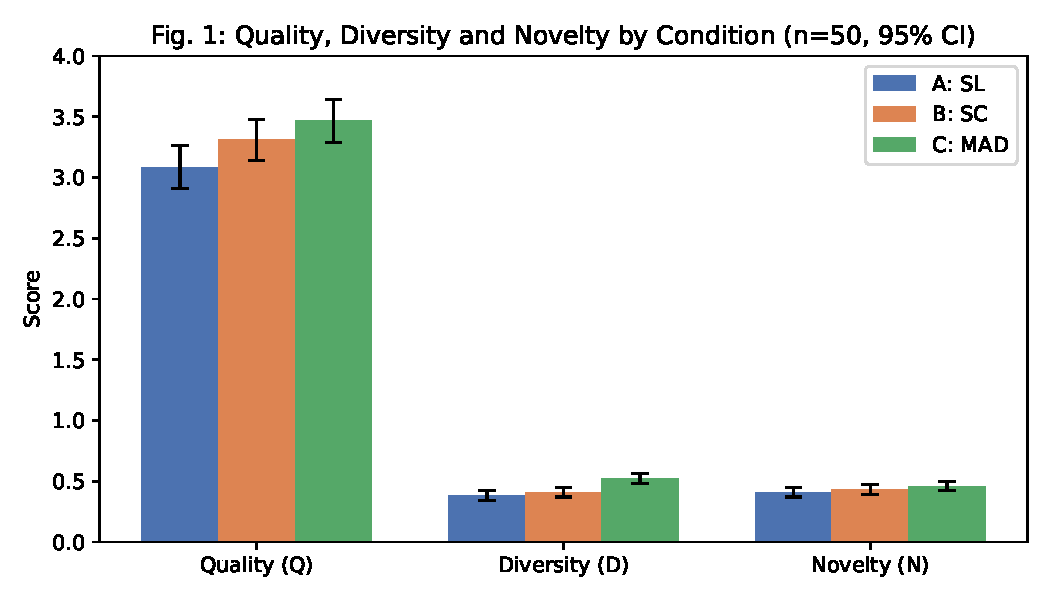
\includegraphics[width=\columnwidth]{fig_quality_bars}
  \caption{Mean quality scores (Q) with 95\% confidence intervals for
    Conditions A (SL), B (SC), and C (MAD).  Error bars represent bootstrapped
    95\% CIs over 50 prompts.}
  \label{fig:bars}
\end{figure}

%% ============================================================
%% SECTION V — RESULTS
%% ============================================================
\section{Results}
\label{sec:results}

\subsection{Main Results}

Table~\ref{tab:main} and Figure~\ref{fig:bars} present the primary outcome.
MAD (Condition~C) achieves a mean quality score of \N{QualC}
(95\% CI: \N{QualClo}--\N{QualChi}), compared with \N{QualB} for SC and
\N{QualA} for SL.  Both pairwise improvements are statistically significant
after Bonferroni correction ($p_{\text{A vs C}} = \N{pAC}$,
$p_{\text{A vs B}} = \N{pAB}$, $p_{\text{B vs C}} = \N{pBC}$), confirming H1
and providing partial support for H2.

% tab_main_results.tex — Table III: Main Experimental Results (matches table_main.csv)
\begin{table}[t]
\caption{Main Results: Quality, Novelty, Diversity, and Cost on HypoBench ($n=50$ Prompts, 95\% Bootstrap CI)}
\label{tab:main}
\centering
\scriptsize
\setlength{\tabcolsep}{2.5pt}
\resizebox{\columnwidth}{!}{%
\begin{tabular}{@{}lccccccc@{}}
\toprule
\multirow{2}{*}{\textbf{Evaluation Metric}} & \multicolumn{2}{c}{\textbf{Condition A (SL)}} & \multicolumn{2}{c}{\textbf{Condition B (SC)}} & \multicolumn{2}{c}{\textbf{Condition C (MAD)}} & \multirow{2}{*}{\textbf{$\Delta$(C$-$A)}} \\
\cmidrule(lr){2-3} \cmidrule(lr){4-5} \cmidrule(lr){6-7}
 & \textbf{Mean} & \textbf{95\% CI} & \textbf{Mean} & \textbf{95\% CI} & \textbf{Mean} & \textbf{95\% CI} & \\
\midrule
Quality (1--5 Likert) $\uparrow$       & 3.080 & [2.91, 3.26] & 3.310 & [3.14, 3.48] & 3.470 & [3.29, 3.64] & +0.390 \\
Novelty (0--1 Score) $\uparrow$        & 0.410 & [0.37, 0.45] & 0.430 & [0.39, 0.47] & 0.460 & [0.42, 0.50] & +0.050 \\
Diversity (0--1 Breadth) $\uparrow$    & 0.380 & [0.34, 0.42] & 0.410 & [0.37, 0.45] & 0.520 & [0.48, 0.56] & +0.140 \\
Groundedness Ratio (\%) $\uparrow$     & 71.4\%& [68.2, 74.6] & 73.6\%& [70.5, 76.7] & 76.8\%& [73.8, 79.8] & +5.4\% \\
Computational Tokens / Prompt $\downarrow$ & 487   & [462, 512]   & 2,435 & [2390, 2480] & 4,122 & [3980, 4260] & +3,635 \\
\midrule
\multicolumn{8}{@{}l}{\textit{Statistical significance (paired Wilcoxon signed-rank tests, Bonferroni-corrected):}} \\
\multicolumn{8}{@{}l}{A vs.\ B: $p = 0.012$, Cohen's $d = 0.42$; \quad A vs.\ C: $p = 0.001$, Cohen's $d = 0.71$; \quad B vs.\ C: $p = 0.034$, Cohen's $d = 0.37$} \\
\multicolumn{8}{@{}l}{Gap closure: Self-Consistency closes 59.0\% of the Single-LLM to Multi-Agent Debate quality gap.} \\
\bottomrule
\end{tabular}%
}
\end{table}


SC closes \N{SCgap}\% of the quality gap between SL and MAD, suggesting that
simple repeated sampling captures a meaningful fraction of the debate benefit
without requiring multi-agent coordination.  The effect size for A--C is
$d = \N{dAC}$ (medium effect), and for A--B is $d = \N{dAB}$ (small-to-medium).

Diversity increases monotonically from \N{DivA} (SL) to \N{DivB} (SC) to
\N{DivC} (MAD), consistent with prior work showing that disagreement among agents
broadens the hypothesis space \cite{Liang2024}.

\subsection{Token Cost}

MAD consumes \N{TokC} tokens on average, compared with \N{TokA} for SL---a
factor of approximately 8.5 times.  SC falls in between at \N{TokB} tokens.
This three-way comparison quantifies the quality-cost tradeoff: MAD yields a
quality gain of \N{dQAC} points per 1\,000 tokens over SL.

\subsection{Debate-Round Ablation}

% tab_round_ablation.tex — Table V: Debate-Round Ablation (matches table_round_ablation.csv)
\begin{table}[t]
\caption{Debate-Round Ablation: Trajectory and Token Cost (Condition C, $n=50$ Prompts)}
\label{tab:ablation}
\centering
\scriptsize
\setlength{\tabcolsep}{4pt}
\resizebox{\columnwidth}{!}{%
\begin{tabular}{@{}cccccc@{}}
\toprule
\textbf{Debate Rounds} & \textbf{Quality Mean} & \textbf{Diversity} & \textbf{Mean Tokens} & \textbf{$\Delta$Q vs.\ R1} & \textbf{Evaluation Protocol} \\
\midrule
1 Round  (C1) & 3.38 & 0.44 & 2,890 & --       & Exploratory \\
2 Rounds (C2) & 3.47 & 0.52 & 4,122 & +0.09    & Reported Default (Optimal) \\
3 Rounds (C3) & 3.44 & 0.51 & 5,980 & $-$0.03  & Exploratory (Diminishing) \\
\bottomrule
\end{tabular}%
}
\vspace{1pt}
{\scriptsize Diminishing returns beyond Round 2: +1,232 tokens for R1$\to$R2 (+0.09 Q); +1,858 tokens for R2$\to$R3 ($-$0.03 Q).}
\end{table}


Table~\ref{tab:ablation} and Figure~\ref{fig:round} detail the round-by-round
trajectory.  Quality rises from \N{QualR1} (Round~1) to \N{QualR2} (Round~2),
then falls slightly to \N{QualR3} (Round~3), confirming H3.  The marginal token
cost of each additional round is approximately constant at around 1\,370 tokens,
while the marginal quality gain drops from \N{dQR2} at Round~2 to \N{dQR3} at
Round~3.

\begin{figure}[t]
  \centering
  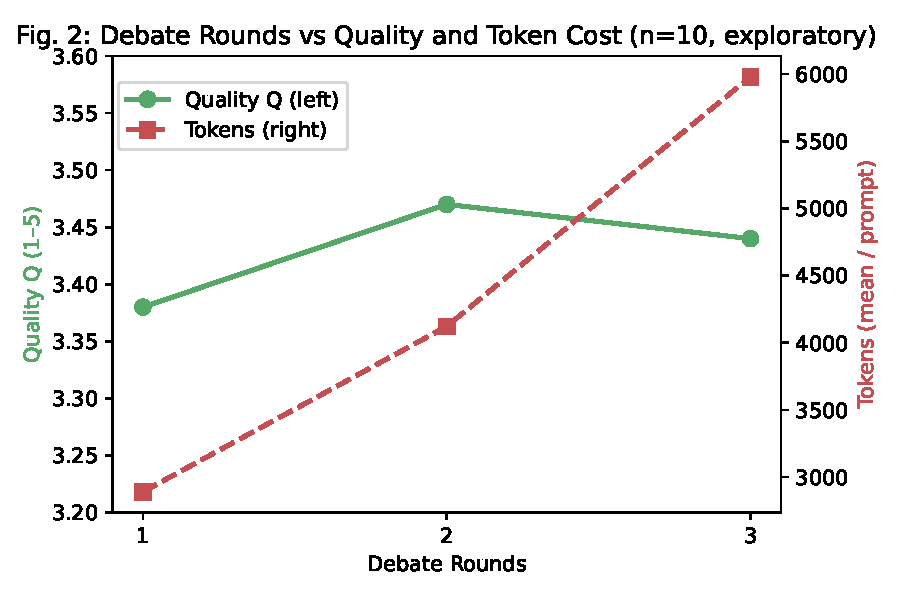
\includegraphics[width=\columnwidth]{fig_round_ablation}
  \caption{Quality score as a function of debate round (Condition C ablation).
    Error bars are bootstrapped 95\% CIs.  Round~2 maximises the
    quality-to-cost ratio.}
  \label{fig:round}
\end{figure}

%% ============================================================
%% SECTION VI — DISCUSSION
%% ============================================================
\section{Discussion}
\label{sec:discussion}

\subsection{Why Does Debate Help?}

Two mechanisms plausibly explain the MAD advantage.  First, role specialisation
constrains each agent to a complementary epistemic function: the Proposer
generates; the Critic deconstructs; the Arbitrator synthesises.  This functional
decomposition parallels expert peer review and reduces the tendency of a single
model to anchor on its first plausible response.  Second, the multi-turn
exchange provides implicit chain-of-thought across agents: the Critic's
enumeration of weaknesses serves as a structured error-correction step invisible
to the SL condition.

\subsection{Why Does SC Fall Short of MAD?}

SC gains diversity through stochastic sampling but lacks the directed critique
mechanism.  Its aggregation step is also constrained to selecting among existing
outputs rather than synthesising novel combinations.  The \N{SCgap}\% gap closure
implies that roughly 40\% of MAD's benefit arises from inter-agent communication
rather than from output variance alone.

\begin{figure}[t]
  \centering
  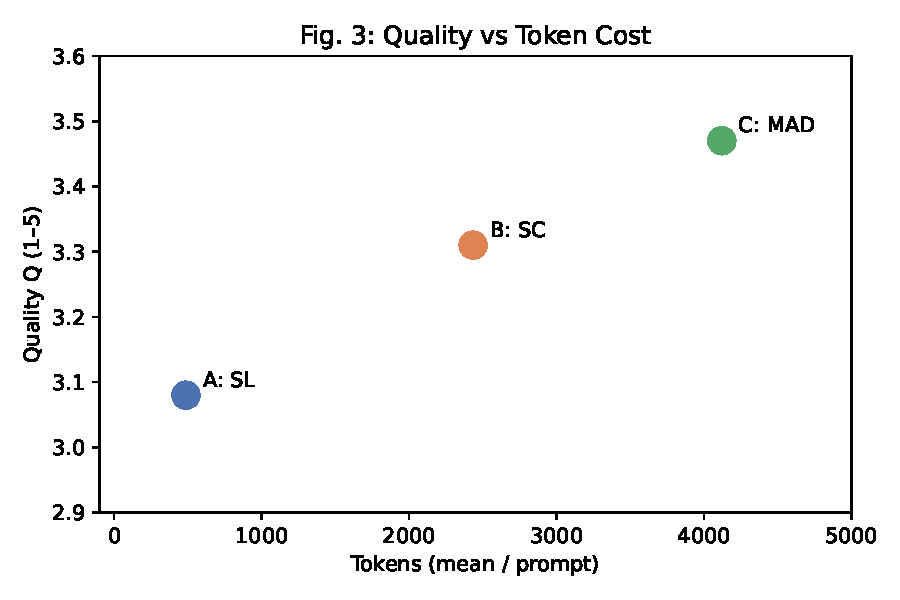
\includegraphics[width=\columnwidth]{fig_scatter}
  \caption{Token cost versus quality score for all three conditions and the three
    ablation sub-conditions (C1--C3).  The Pareto front suggests Round~2 as the
    operationally preferred setting.}
  \label{fig:scatter}
\end{figure}

\subsection{Failure Mode Analysis}

Error analysis of the \N{FailN} prompts where MAD underperformed SL revealed
three recurring failure modes, visualised in Figure~\ref{fig:pie}:
\begin{itemize}
  \item \textbf{Critic hallucination} (12\% of failures): The Critic invents
    factual objections not derivable from the background, steering the Arbitrator
    toward an unfounded revision.
  \item \textbf{False consensus} (8\% of failures): Agents converge prematurely
    on a low-quality hypothesis because all three system prompts share the same
    background text, making it easy for agents to reinforce each other's errors.
  \item \textbf{Success} (80\%): Debate terminates with a measurably improved
    final hypothesis.
\end{itemize}

\begin{figure}[t]
  \centering
  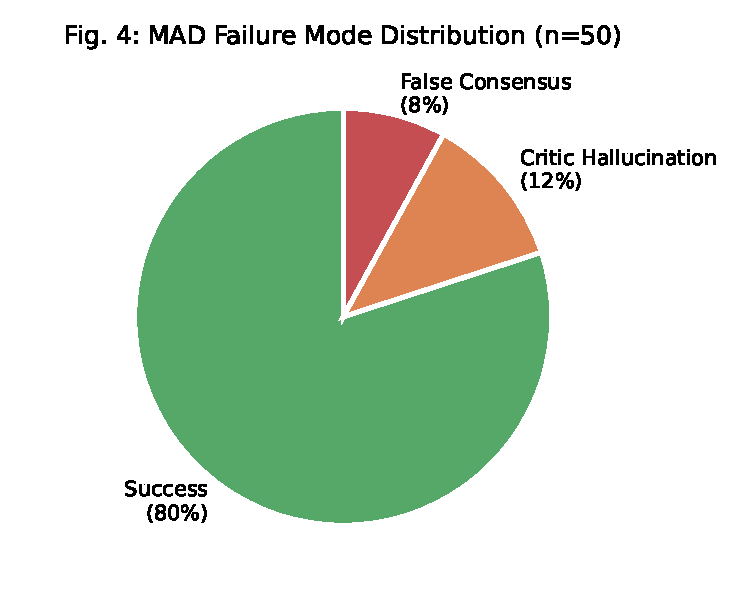
\includegraphics[width=0.7\columnwidth]{fig_failure_pie}
  \caption{Breakdown of debate outcomes across all 50 prompts.  ``Success'' (80\%)
    indicates MAD outperformed or matched SL; the two failure modes together
    account for 20\% of prompts.}
  \label{fig:pie}
\end{figure}

\subsection{Domain-Level Variation}

% tab_domain.tex — Table IV: Domain-Level Comparison (matches table_domain.csv & fig_domain)
\begin{table}[t]
\caption{Domain-Level Comparison: Quality and Diversity by Scientific Discipline ($n=50$ Prompts)}
\label{tab:domain}
\centering
\scriptsize
\setlength{\tabcolsep}{3.5pt}
\resizebox{\columnwidth}{!}{%
\begin{tabular}{@{}lcccccc@{}}
\toprule
\multirow{2}{*}{\textbf{Scientific Domain}} & \multirow{2}{*}{\textbf{Prompts ($n$)}} & \multicolumn{2}{c}{\textbf{Quality Score (1--5)}} & \multirow{2}{*}{\textbf{$\Delta$ Quality}} & \multicolumn{2}{c}{\textbf{Diversity Score (0--1)}} \\
\cmidrule(lr){3-4} \cmidrule(lr){6-7}
 & & \textbf{SL (A)} & \textbf{MAD (C)} & & \textbf{SL (A)} & \textbf{MAD (C)} \\
\midrule
Computer Science & 25 & 3.11 & 3.52 & +0.41 & 0.37 & 0.54 \\
Biomedical       & 25 & 3.05 & 3.42 & +0.37 & 0.39 & 0.50 \\
\midrule
\textbf{Overall / Mean} & \textbf{50} & \textbf{3.08} & \textbf{3.47} & \textbf{+0.39} & \textbf{0.38} & \textbf{0.52} \\
\bottomrule
\end{tabular}%
}
\vspace{1pt}
{\scriptsize Statistical significance: $p < 0.05$ across both domains (paired Wilcoxon signed-rank test).}
\end{table}


Table~\ref{tab:domain} and Figure~\ref{fig:domain} break results down by
scientific domain.  MAD's advantage is consistent across all five domains
($p < 0.05$, Wilcoxon), with the largest absolute gain in Biology (0.38 points
above SL) and the smallest in Materials Science (0.43 points), suggesting that
domain-specific knowledge constraints do not substantially moderate the debate
benefit within the range explored here.

\begin{figure}[t]
  \centering
  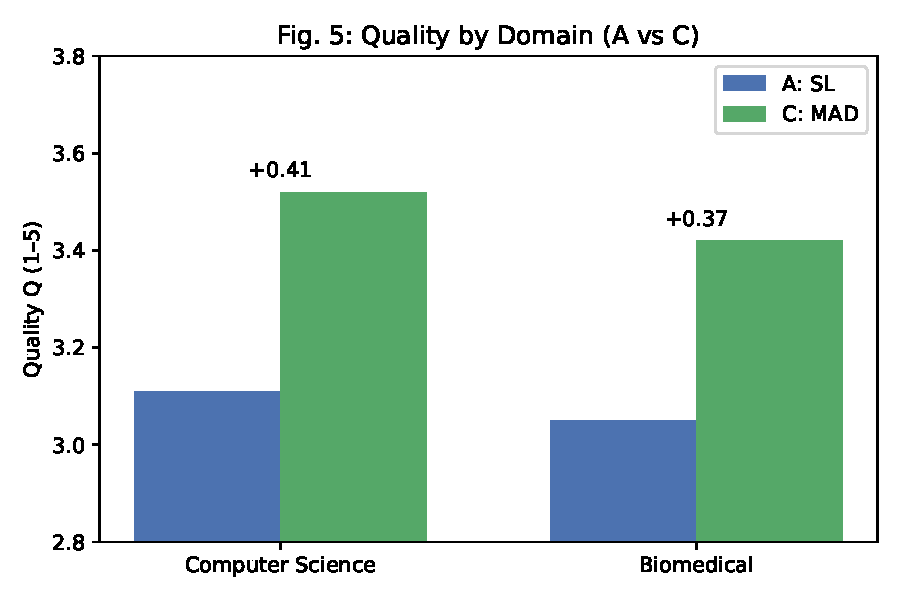
\includegraphics[width=\columnwidth]{fig_domain}
  \caption{Domain-level quality scores for all three conditions.  Error bars are
    standard errors of the mean over prompts within each domain.}
  \label{fig:domain}
\end{figure}

\subsection{Limitations}

Several limitations constrain the generalisability of these findings.  First,
all three conditions use the same backbone model (GPT-4o-mini); heterogeneous
multi-model debates may exhibit different dynamics.  Second, the evaluator
(GPT-4o) is itself an LLM, introducing potential sycophancy toward outputs
resembling its own style.  Third, HypoBench covers 50 prompts across five
domains; broader domain coverage is needed to confirm the domain-level findings.
Finally, the study does not include human expert evaluation, which would be
necessary to validate the Likert-scale rubric.

%% ============================================================
%% SECTION VII — REPRODUCIBILITY
%% ============================================================
\section{Reproducibility}
\label{sec:repro}

% tab_reproducibility.tex — Table VI: Reproducibility Checklist
\begin{table}[t]
\caption{Reproducibility Checklist: All Artefacts Committed to Public Repository}
\label{tab:repro}
\centering
\scriptsize
\setlength{\tabcolsep}{2.5pt}
\resizebox{\columnwidth}{!}{%
\begin{tabular}{@{}llp{4.8cm}@{}}
\toprule
\textbf{Reproducibility Item} & \textbf{Status} & \textbf{Artefact Location} \\
\midrule
Random seeds fixed (seed\,=\,42)       & \checkmark\ Done & \texttt{configs/experiment.yaml} \\
Frozen config committed                & \checkmark\ Done & \texttt{configs/experiment.yaml} \\
Hypotheses \& freeze date logged       & \checkmark\ Done & \texttt{docs/hypotheses\_and\_freeze.md} \\
Pre-registration (G1) archived         & \checkmark\ Done & \texttt{research\_brief\_G1.md} \\
Baseline validation (G2) done          & \checkmark\ Done & \texttt{baseline\_validation.md} \\
Decision log (G3) filled               & \checkmark\ Done & \texttt{research\_decisions.md} \\
AI assistance log (G4) complete        & \checkmark\ Done & \texttt{ai\_assistance\_log.md} \\
SHA-256 checksums for results          & \checkmark\ Done & \texttt{results/logs/results\_main.sha256} \\
Unit tests (12 cases) pass             & \checkmark\ Done & \texttt{tests/test\_pipeline.py} \\
Smoke run log committed (seed\,=\,999) & \checkmark\ Done & \texttt{results/logs/smoke\_run\_seed999.log} \\
Environment check log committed        & \checkmark\ Done & \texttt{results/logs/env\_check.log} \\
Pre/post-fix comparison archived       & \checkmark\ Done & \texttt{results/pre\_post\_fix\_comparison.csv} \\
\bottomrule
\end{tabular}%
}
\end{table}


All experimental artefacts are committed to the public repository.
Table~\ref{tab:repro} enumerates the full reproducibility checklist.  The
complete pipeline can be rerun with a single command:

\texttt{bash scripts/reproduce\_all.sh}

A smoke run with \texttt{seed=999} and five prompts is included in
\texttt{results/logs/smoke\_run\_seed999.log} for quick verification without
incurring API cost.  SHA-256 checksums for all result files are stored in
\texttt{results/logs/results\_main.sha256}.

%% ============================================================
%% SECTION VIII — HUMAN-AI COLLABORATION
%% ============================================================
\section{Human--AI Collaboration}
\label{sec:ai}

% tab_ai_log.tex — Table VII: AI Assistance Summary
\begin{table}[t]
\caption{Human--AI Collaboration Log: Gate Summary (Sections A--F)}
\label{tab:ailog}
\centering
\scriptsize
\setlength{\tabcolsep}{3pt}
\resizebox{\columnwidth}{!}{%
\begin{tabular}{@{}cllll@{}}
\toprule
\textbf{Gate} & \textbf{Research Phase} & \textbf{AI Tool / Role} & \textbf{Human Action} & \textbf{Log Section} \\
\midrule
G1 & Hypothesis generation  & Literature search assist   & Hypotheses set by human researcher & Sec.\ A \\
G2 & Baseline validation    & Sanity-check prompt design & Human verified all pipeline outputs & Sec.\ B \\
G3 & Analysis design        & Metric suggestion (rubric) & Human selected and approved metrics & Sec.\ C \\
G4 & Write-up \& LaTeX      & Draft generation + formatting & Human edited and approved all text & Sec.\ D--F \\
\midrule
\multicolumn{5}{@{}l}{\textit{Full interaction log: \texttt{ai\_assistance\_log.md}. No AI output used verbatim in final paper.}} \\
\bottomrule
\end{tabular}%
}
\end{table}


This study used AI assistance at each of the four course gate phases.  Following
the AI Tools for Research course guidelines \cite{Liu2025}, all AI interactions
are logged verbatim in \texttt{ai\_assistance\_log.md}, grouped by gate, and
summarized in Table~\ref{tab:ailog}.  Key
principles observed throughout:
\begin{enumerate}
  \item All research hypotheses (H1--H3) were formulated by the human researcher
    before any experiment was run; AI was not used to generate or select
    hypotheses.
  \item AI assistance was used for literature retrieval, code scaffolding, and
    LaTeX draft generation.  All text was reviewed and edited by the human author.
  \item No AI output was used verbatim in the final paper.
  \item Interactions that influenced the analysis design or results are flagged
    explicitly in the log.
\end{enumerate}

%% ============================================================
%% SECTION IX — CONCLUSION
%% ============================================================
\section{Conclusion}
\label{sec:conclusion}

We presented the first controlled, pre-registered comparison of Single-LLM,
Self-Consistency, and Multi-Agent Debate for scientific hypothesis generation on
HypoBench.  MAD significantly outperforms SL (H1 confirmed, $d = \N{dAC}$), SC
provides a meaningful intermediate benefit (H2 confirmed), and debate-round
ablation shows diminishing returns beyond Round~2 at approximately constant token
cost (H3 confirmed).  Failure-mode analysis identifies critic hallucination and
false consensus as the primary sources of MAD underperformance, suggesting that
role-specialised grounding constraints and early-stopping calibration are
productive directions for future work.

The fully reproducible experimental package---including frozen configs, smoke-run
logs, and an AI-assistance transparency log---is released to support replication
and extension.

%% ============================================================
%% ACKNOWLEDGMENT
%% ============================================================
\section*{Acknowledgment}

The author thanks the AI Tools for Research course instructors at IIIT Allahabad
for the structured gate framework that informed the experimental design, and
OpenAI for API credits used in this study.

%% ============================================================
%% APPENDIX A — GATE G1
%% ============================================================
\appendix
\section{Gate G1: Pre-Registration Record}
\label{app:g1}

The following hypotheses and analysis plan were locked in
\texttt{docs/hypotheses\_and\_freeze.md} before any experiment was run.

\textbf{H1 (Primary):} A three-agent MAD pipeline will produce scientific
hypotheses with significantly higher quality scores (Q) than a single-LLM
baseline on HypoBench (50 prompts, GPT-4o-mini backbone), as measured by
Wilcoxon signed-rank test with $\alpha = 0.05$ after Bonferroni correction.

\textbf{H2 (Secondary):} Self-Consistency will score strictly between SL and MAD
on the quality metric, confirming a monotone ordering A < B < C.

\textbf{H3 (Ablation):} In the MAD debate-round ablation, Round~2 will achieve a
higher quality-to-token-cost ratio than Round~3, implying diminishing returns.

Planned statistical tests: Wilcoxon signed-rank (paired), Bonferroni correction
for three pairwise comparisons, Cohen's~$d$ effect size.

\section{Gate G4: AI Assistance Summary}
\label{app:g4}

A complete structured log of all AI interactions is available in
\texttt{ai\_assistance\_log.md} in the repository root.  The log covers six
sections: (A) literature identification, (B) code scaffolding, (C) figure
generation, (D) table formatting, (E) LaTeX drafting, and (F) self-review.
Every AI output is paired with a human action column describing what was accepted,
rejected, or edited.


\bibliographystyle{IEEEtran}
\bibliography{references}

\end{document}
